\documentclass{standalone}
\usepackage{tikz}
\usetikzlibrary{shapes.geometric}
\usetikzlibrary{patterns, positioning}


\begin{document}
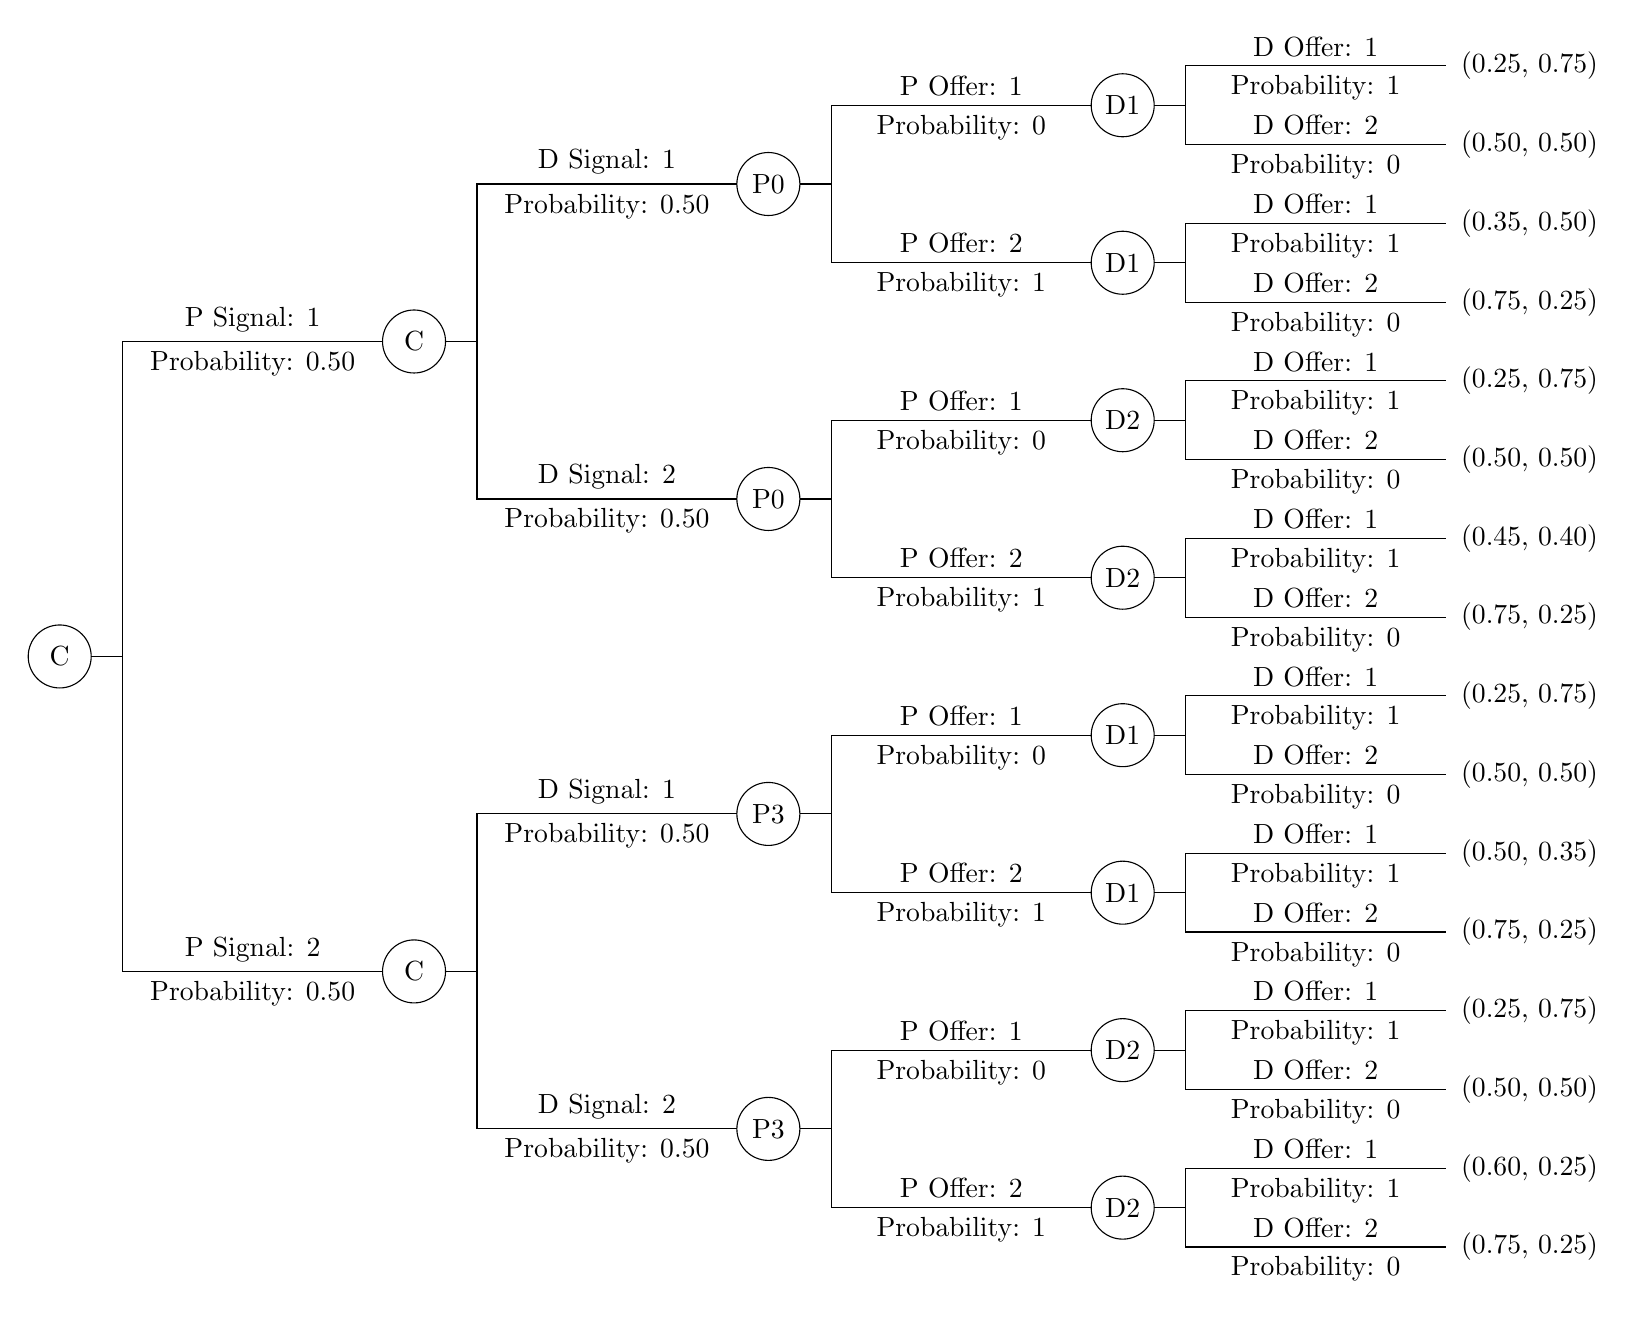
\begin{tikzpicture}

    \draw[color=black] (-18, -7.75) circle (0.4cm) node[draw=none] (N0) {C};

    \draw[color=black] (-13.5, -3.75) circle (0.4cm) node[draw=none] (N0) {C};
\draw (-17.6, -7.75) -- (-17.200000000000003, -7.75) -- (-17.200000000000003, -3.75) -- (-13.9, -3.75) node [midway, above, sloped] (E0) {P Signal: 1} node [midway, below, sloped] (E1) {Probability: 0.50} ;


    \draw[color=black] (-9, -1.75) circle (0.4cm) node[draw=none] (N2) {P0};
\draw (-13.1, -3.75) -- (-12.7, -3.75) -- (-12.7, -1.75) -- (-9.4, -1.75) node [midway, above, sloped] (E2) {D Signal: 1} node [midway, below, sloped] (E3) {Probability: 0.50} ;


    \draw[color=black] (-4.5, -0.75) circle (0.4cm) node[draw=none] (N4) {D1};
\draw (-8.6, -1.75) -- (-8.2, -1.75) -- (-8.2, -0.75) -- (-4.9, -0.75) node [midway, above, sloped] (E4) {P Offer: 1} node [midway, below, sloped] (E5) {Probability: 0} ;


    \draw[color=black] (0, -0.25) node[draw=none] (N6) {};
\node[draw=none, right=-0.45cm of N6] {(0.25, 0.75)};
\draw (-4.1, -0.75) -- (-3.6999999999999997, -0.75) -- (-3.6999999999999997, -0.25) -- (-0.4, -0.25) node [midway, above, sloped] (E6) {D Offer: 1} node [midway, below, sloped] (E7) {Probability: 1} ;


    \draw[color=black] (0, -1.25) node[draw=none] (N8) {};
\node[draw=none, right=-0.45cm of N8] {(0.50, 0.50)};
\draw (-4.1, -0.75) -- (-3.6999999999999997, -0.75) -- (-3.6999999999999997, -1.25) -- (-0.4, -1.25) node [midway, above, sloped] (E8) {D Offer: 2} node [midway, below, sloped] (E9) {Probability: 0} ;


    \draw[color=black] (-4.5, -2.75) circle (0.4cm) node[draw=none] (N10) {D1};
\draw (-8.6, -1.75) -- (-8.2, -1.75) -- (-8.2, -2.75) -- (-4.9, -2.75) node [midway, above, sloped] (E10) {P Offer: 2} node [midway, below, sloped] (E11) {Probability: 1} ;


    \draw[color=black] (0, -2.25) node[draw=none] (N12) {};
\node[draw=none, right=-0.45cm of N12] {(0.35, 0.50)};
\draw (-4.1, -2.75) -- (-3.6999999999999997, -2.75) -- (-3.6999999999999997, -2.25) -- (-0.4, -2.25) node [midway, above, sloped] (E12) {D Offer: 1} node [midway, below, sloped] (E13) {Probability: 1} ;


    \draw[color=black] (0, -3.25) node[draw=none] (N14) {};
\node[draw=none, right=-0.45cm of N14] {(0.75, 0.25)};
\draw (-4.1, -2.75) -- (-3.6999999999999997, -2.75) -- (-3.6999999999999997, -3.25) -- (-0.4, -3.25) node [midway, above, sloped] (E14) {D Offer: 2} node [midway, below, sloped] (E15) {Probability: 0} ;


    \draw[color=black] (-9, -5.75) circle (0.4cm) node[draw=none] (N16) {P0};
\draw (-13.1, -3.75) -- (-12.7, -3.75) -- (-12.7, -5.75) -- (-9.4, -5.75) node [midway, above, sloped] (E16) {D Signal: 2} node [midway, below, sloped] (E17) {Probability: 0.50} ;


    \draw[color=black] (-4.5, -4.75) circle (0.4cm) node[draw=none] (N18) {D2};
\draw (-8.6, -5.75) -- (-8.2, -5.75) -- (-8.2, -4.75) -- (-4.9, -4.75) node [midway, above, sloped] (E18) {P Offer: 1} node [midway, below, sloped] (E19) {Probability: 0} ;


    \draw[color=black] (0, -4.25) node[draw=none] (N20) {};
\node[draw=none, right=-0.45cm of N20] {(0.25, 0.75)};
\draw (-4.1, -4.75) -- (-3.6999999999999997, -4.75) -- (-3.6999999999999997, -4.25) -- (-0.4, -4.25) node [midway, above, sloped] (E20) {D Offer: 1} node [midway, below, sloped] (E21) {Probability: 1} ;


    \draw[color=black] (0, -5.25) node[draw=none] (N22) {};
\node[draw=none, right=-0.45cm of N22] {(0.50, 0.50)};
\draw (-4.1, -4.75) -- (-3.6999999999999997, -4.75) -- (-3.6999999999999997, -5.25) -- (-0.4, -5.25) node [midway, above, sloped] (E22) {D Offer: 2} node [midway, below, sloped] (E23) {Probability: 0} ;


    \draw[color=black] (-4.5, -6.75) circle (0.4cm) node[draw=none] (N24) {D2};
\draw (-8.6, -5.75) -- (-8.2, -5.75) -- (-8.2, -6.75) -- (-4.9, -6.75) node [midway, above, sloped] (E24) {P Offer: 2} node [midway, below, sloped] (E25) {Probability: 1} ;


    \draw[color=black] (0, -6.25) node[draw=none] (N26) {};
\node[draw=none, right=-0.45cm of N26] {(0.45, 0.40)};
\draw (-4.1, -6.75) -- (-3.6999999999999997, -6.75) -- (-3.6999999999999997, -6.25) -- (-0.4, -6.25) node [midway, above, sloped] (E26) {D Offer: 1} node [midway, below, sloped] (E27) {Probability: 1} ;


    \draw[color=black] (0, -7.25) node[draw=none] (N28) {};
\node[draw=none, right=-0.45cm of N28] {(0.75, 0.25)};
\draw (-4.1, -6.75) -- (-3.6999999999999997, -6.75) -- (-3.6999999999999997, -7.25) -- (-0.4, -7.25) node [midway, above, sloped] (E28) {D Offer: 2} node [midway, below, sloped] (E29) {Probability: 0} ;


    \draw[color=black] (-13.5, -11.75) circle (0.4cm) node[draw=none] (N30) {C};
\draw (-17.6, -7.75) -- (-17.200000000000003, -7.75) -- (-17.200000000000003, -11.75) -- (-13.9, -11.75) node [midway, above, sloped] (E30) {P Signal: 2} node [midway, below, sloped] (E31) {Probability: 0.50} ;


    \draw[color=black] (-9, -9.75) circle (0.4cm) node[draw=none] (N32) {P3};
\draw (-13.1, -11.75) -- (-12.7, -11.75) -- (-12.7, -9.75) -- (-9.4, -9.75) node [midway, above, sloped] (E32) {D Signal: 1} node [midway, below, sloped] (E33) {Probability: 0.50} ;


    \draw[color=black] (-4.5, -8.75) circle (0.4cm) node[draw=none] (N34) {D1};
\draw (-8.6, -9.75) -- (-8.2, -9.75) -- (-8.2, -8.75) -- (-4.9, -8.75) node [midway, above, sloped] (E34) {P Offer: 1} node [midway, below, sloped] (E35) {Probability: 0} ;


    \draw[color=black] (0, -8.25) node[draw=none] (N36) {};
\node[draw=none, right=-0.45cm of N36] {(0.25, 0.75)};
\draw (-4.1, -8.75) -- (-3.6999999999999997, -8.75) -- (-3.6999999999999997, -8.25) -- (-0.4, -8.25) node [midway, above, sloped] (E36) {D Offer: 1} node [midway, below, sloped] (E37) {Probability: 1} ;


    \draw[color=black] (0, -9.25) node[draw=none] (N38) {};
\node[draw=none, right=-0.45cm of N38] {(0.50, 0.50)};
\draw (-4.1, -8.75) -- (-3.6999999999999997, -8.75) -- (-3.6999999999999997, -9.25) -- (-0.4, -9.25) node [midway, above, sloped] (E38) {D Offer: 2} node [midway, below, sloped] (E39) {Probability: 0} ;


    \draw[color=black] (-4.5, -10.75) circle (0.4cm) node[draw=none] (N40) {D1};
\draw (-8.6, -9.75) -- (-8.2, -9.75) -- (-8.2, -10.75) -- (-4.9, -10.75) node [midway, above, sloped] (E40) {P Offer: 2} node [midway, below, sloped] (E41) {Probability: 1} ;


    \draw[color=black] (0, -10.25) node[draw=none] (N42) {};
\node[draw=none, right=-0.45cm of N42] {(0.50, 0.35)};
\draw (-4.1, -10.75) -- (-3.6999999999999997, -10.75) -- (-3.6999999999999997, -10.25) -- (-0.4, -10.25) node [midway, above, sloped] (E42) {D Offer: 1} node [midway, below, sloped] (E43) {Probability: 1} ;


    \draw[color=black] (0, -11.25) node[draw=none] (N44) {};
\node[draw=none, right=-0.45cm of N44] {(0.75, 0.25)};
\draw (-4.1, -10.75) -- (-3.6999999999999997, -10.75) -- (-3.6999999999999997, -11.25) -- (-0.4, -11.25) node [midway, above, sloped] (E44) {D Offer: 2} node [midway, below, sloped] (E45) {Probability: 0} ;


    \draw[color=black] (-9, -13.75) circle (0.4cm) node[draw=none] (N46) {P3};
\draw (-13.1, -11.75) -- (-12.7, -11.75) -- (-12.7, -13.75) -- (-9.4, -13.75) node [midway, above, sloped] (E46) {D Signal: 2} node [midway, below, sloped] (E47) {Probability: 0.50} ;


    \draw[color=black] (-4.5, -12.75) circle (0.4cm) node[draw=none] (N48) {D2};
\draw (-8.6, -13.75) -- (-8.2, -13.75) -- (-8.2, -12.75) -- (-4.9, -12.75) node [midway, above, sloped] (E48) {P Offer: 1} node [midway, below, sloped] (E49) {Probability: 0} ;


    \draw[color=black] (0, -12.25) node[draw=none] (N50) {};
\node[draw=none, right=-0.45cm of N50] {(0.25, 0.75)};
\draw (-4.1, -12.75) -- (-3.6999999999999997, -12.75) -- (-3.6999999999999997, -12.25) -- (-0.4, -12.25) node [midway, above, sloped] (E50) {D Offer: 1} node [midway, below, sloped] (E51) {Probability: 1} ;


    \draw[color=black] (0, -13.25) node[draw=none] (N52) {};
\node[draw=none, right=-0.45cm of N52] {(0.50, 0.50)};
\draw (-4.1, -12.75) -- (-3.6999999999999997, -12.75) -- (-3.6999999999999997, -13.25) -- (-0.4, -13.25) node [midway, above, sloped] (E52) {D Offer: 2} node [midway, below, sloped] (E53) {Probability: 0} ;


    \draw[color=black] (-4.5, -14.75) circle (0.4cm) node[draw=none] (N54) {D2};
\draw (-8.6, -13.75) -- (-8.2, -13.75) -- (-8.2, -14.75) -- (-4.9, -14.75) node [midway, above, sloped] (E54) {P Offer: 2} node [midway, below, sloped] (E55) {Probability: 1} ;


    \draw[color=black] (0, -14.25) node[draw=none] (N56) {};
\node[draw=none, right=-0.45cm of N56] {(0.60, 0.25)};
\draw (-4.1, -14.75) -- (-3.6999999999999997, -14.75) -- (-3.6999999999999997, -14.25) -- (-0.4, -14.25) node [midway, above, sloped] (E56) {D Offer: 1} node [midway, below, sloped] (E57) {Probability: 1} ;


    \draw[color=black] (0, -15.25) node[draw=none] (N58) {};
\node[draw=none, right=-0.45cm of N58] {(0.75, 0.25)};
\draw (-4.1, -14.75) -- (-3.6999999999999997, -14.75) -- (-3.6999999999999997, -15.25) -- (-0.4, -15.25) node [midway, above, sloped] (E58) {D Offer: 2} node [midway, below, sloped] (E59) {Probability: 0} ;


\end{tikzpicture}
\end{document}